\section{Algorithm: Model--Harness Co-design and Recursive Self-Improvement}
\label{sec:algorithm}

An LLM agent emits text; a harness turns that text into actions~\citep{wu2026replharnesses}. Everything visible to the user, what tools exist, how a UI renders, how a tool result is fed back into the model, lives in this layer. In \macaron{} the harness is a first-class training target: we treat train--serve harness divergence as a bug to fix at the source rather than as a modeling problem to paper over~\citep{macaron_v1_preview2026}. The harness defines the action interface and the runtime contract the model is trained against; the recursive self-improvement loop then optimizes the model--harness pair over that contract. This section describes the two halves together: first the harness components, then the RSI cycle that runs against them.

\subsection{Model--Harness Co-design}
\label{sec:harness}
\label{sec:harness_matters}

A harness is the substrate that determines how much of an agent's computation can be \emph{executed} rather than \emph{re-described}~\citep{wu2026replharnesses,codeact2024}. Discrete substrates like one-JSON-tool-per-turn~\citep{patil2025berkeley} force every intermediate value back through the model as text; expressive substrates keep computation in a state the model never restates. Holding model, tasks, primitives, and budgets fixed, changing only the substrate changes both success rate and token cost, sometimes by large factors~\citep{wu2026replharnesses}.

Two design commitments follow from this observation and shape everything in this subsection:
\begin{itemize}[leftmargin=*]
  \item \textbf{The harness should get lighter as the model gets stronger.} A brittle schema that carries the model is a ceiling. A harness that expresses ordinary programmer-shaped code lets a general model do most of the work, and reserves specialist adapters for judgment calls~\citep{ui4a2026}.
  \item \textbf{Training and serving share an explicit runtime contract.} \mindforge{} (Section~\ref{sec:rsi}) records the HCP and action substrate used by an evaluation backend. Reusing those artifacts makes configuration drift visible; the backend remains responsible for reproducing the production tool surface.
\end{itemize}

\subsubsection{\uifora: A Component-Native Harness for Generative UI}
\label{sec:harness_ui4a}

Generative UI~\citep{leviathan2025generative,chen2025generative} has historically been approached in two ways, each with a ceiling (Figure~\ref{fig:ui4a_comparison}).
\begin{itemize}[leftmargin=*]
  \item \textbf{HTML-native.} Maximum expressiveness, minimum control~\citep{si2025design2code}; the harness inherits every compiler, bundler, and error-recovery problem of raw web development.
  \item \textbf{Schema-native.} Verifiable and auditable but capped by the catalog~\citep{a2ui_v08,macaron_a2ui2026}. The schema's ceiling caps the model's ceiling.
\end{itemize}
Our prior schema-native work (Macaron-A2UI~\citep{macaron_a2ui2026}) taught us the point that most affects a shipping agent: teaching the model \emph{when} to render a UI matters more than teaching it \emph{how}.

\begin{figure}[t]
  \centering
  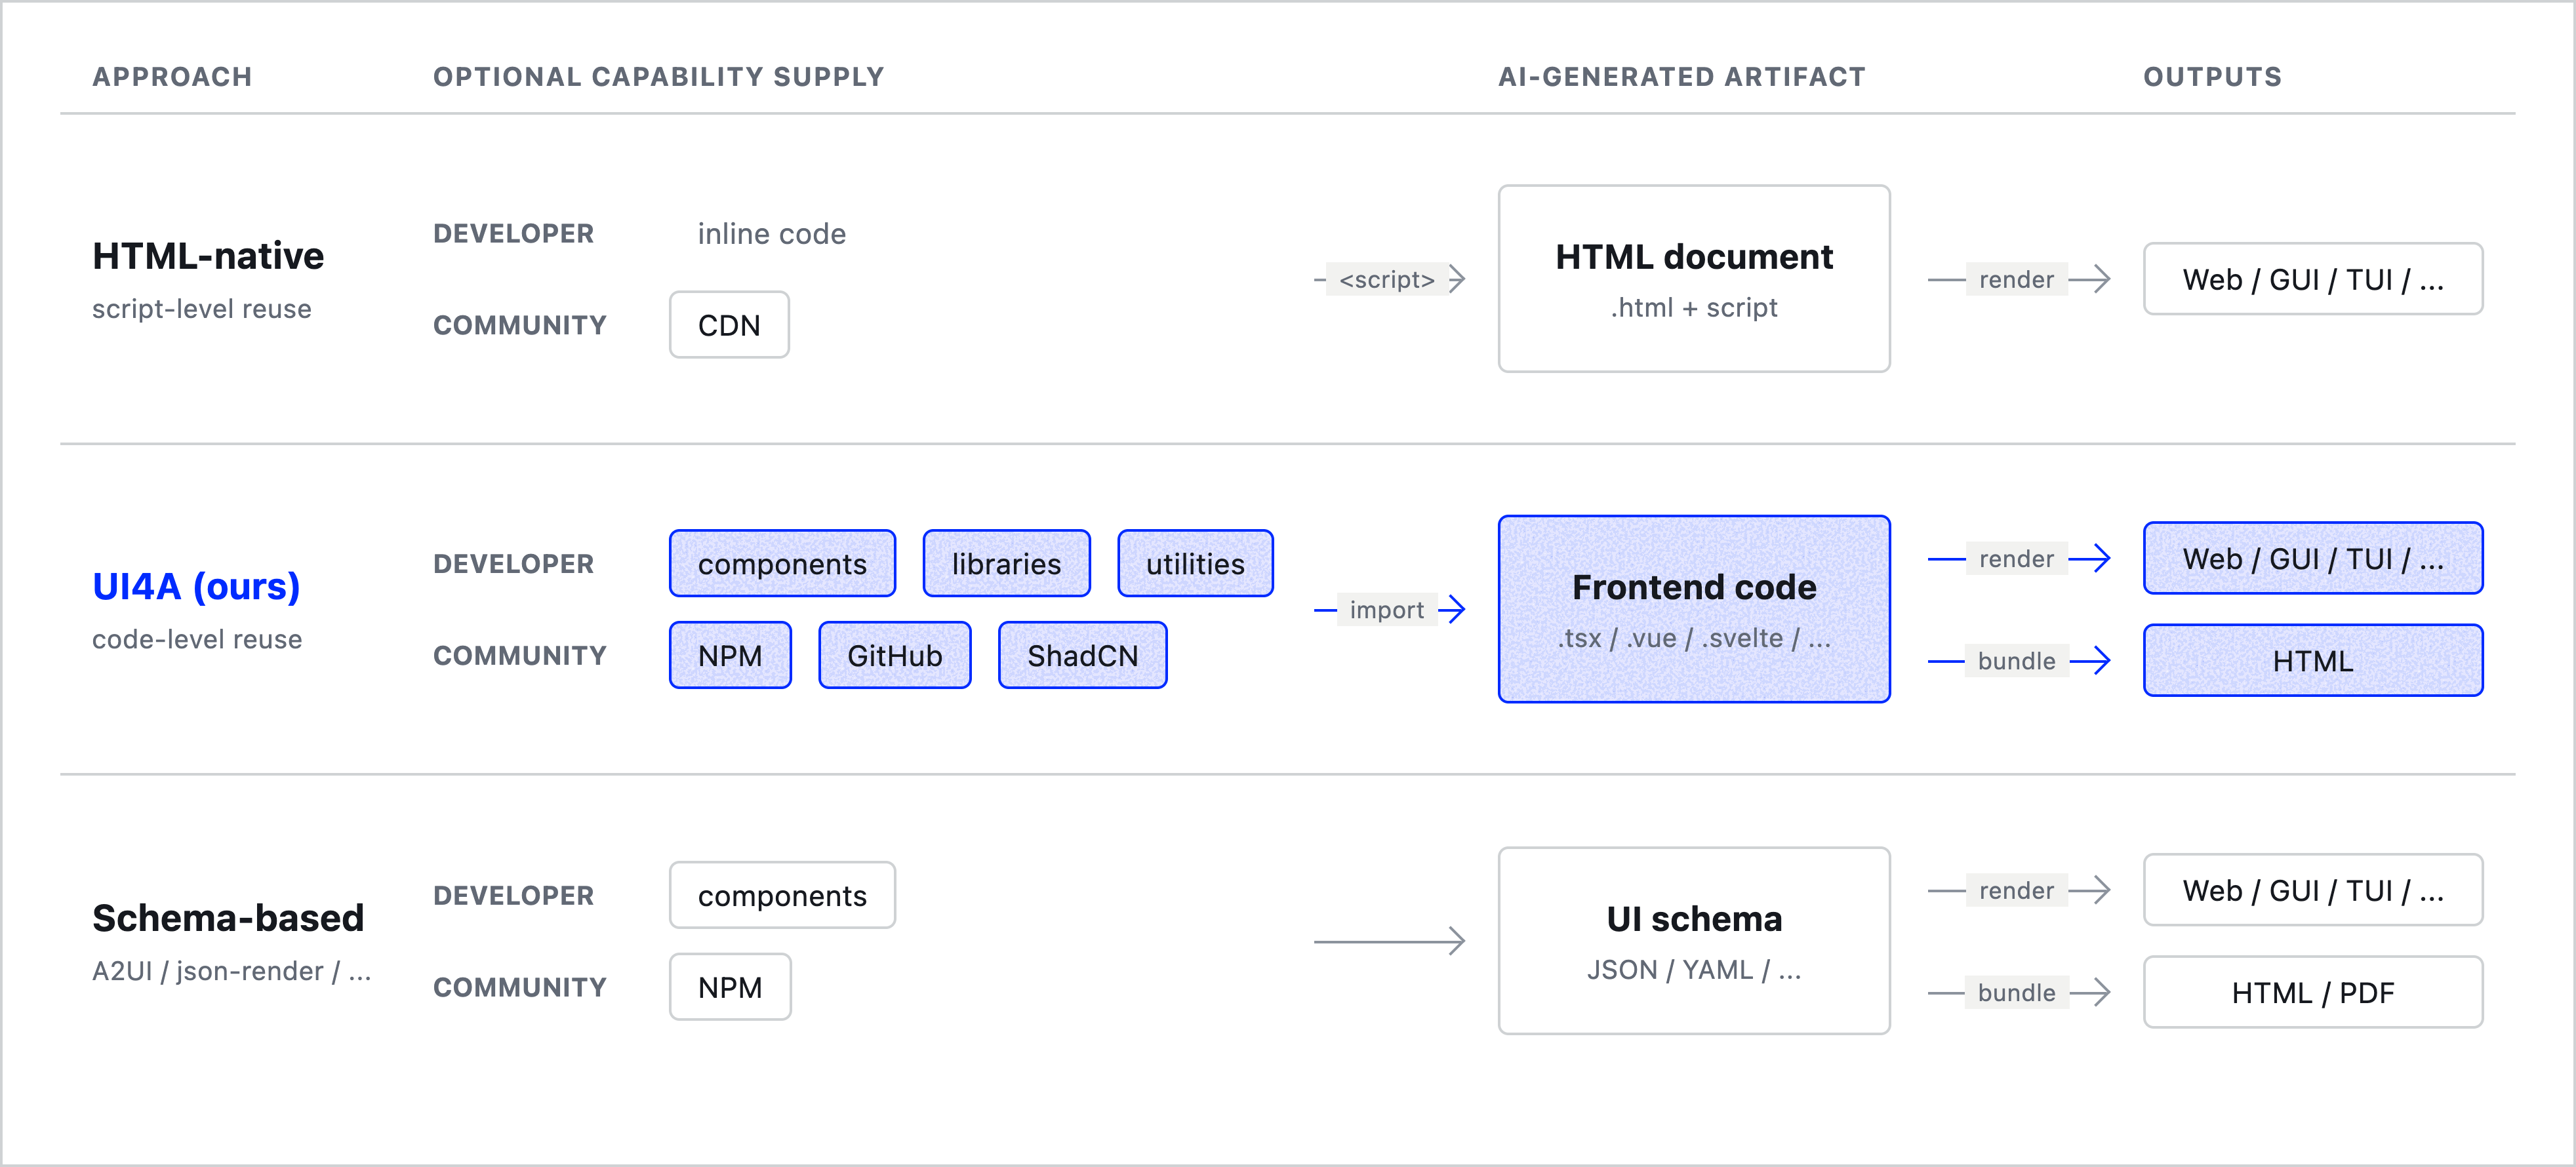
\includegraphics[width=0.95\textwidth]{figures/ui4a_comparison.png}
  \caption{Three approaches to generative UI. HTML-native maximizes expressiveness but inherits raw web development's failure modes; schema-native is verifiable but capped by the component catalog; \uifora{} (component-native) lets the model write ordinary frontend code under runtime-enforced boundaries, recovering expressiveness without the schema ceiling.}
  \label{fig:ui4a_comparison}
\end{figure}

\begin{figure}[t]
  \centering
  
\includegraphics[width=\textwidth]{figures/ui4a_gallery.png}
  \caption{A slice of the \uifora{}-Bench gallery. Each card is generated as ordinary frontend code under runtime-enforced boundaries; \uifora{}-Bench scores them on compile/render correctness, control wiring, and screen fit. The L3 specialist decides \emph{when} to render; the substrate carries \emph{how}.}
  \label{fig:genui_cases}
\end{figure}

\uifora{}~\citep{ui4a2026} is \macaron's component-native answer. The agent writes ordinary frontend code with imports, components, state, and functions, inside runtime-enforced boundaries. Its mental model is \emph{import + component + state + Action}:
\begin{itemize}[leftmargin=*]
  \item \textbf{Import.} The agent pulls components from a curated Macaron registry or common ecosystem primitives (Radix, shadcn, Recharts, KaTeX, lucide-react), with raw HTML/CSS available when a case demands it.
  \item \textbf{Component and state.} Ordinary frontend code the model already knows how to write; no proprietary schema envelope.
  \item \textbf{Action contract.} Every user gesture is a structured object with four fields: \emph{Origin} (which surface), \emph{State} (what data it read), \emph{Execution} (local function or agent event), and \emph{Visibility} (including a \verb|NoAI| boundary for fields the model must not see). The runtime decides whether to run locally, prompt the user, or dispatch as an agent event.
\end{itemize}

Two axes of flexibility follow. The agent can scale \emph{down} to the curated registry for efficiency, or scale \emph{up} to arbitrary frontend code (LaTeX, 3D, generative visuals) when the case genuinely requires it~\citep{ui4a2026}. Rendering is framework-agnostic: React, Vue, Svelte, and SolidJS render from the same output; adding a target ships a small renderer rather than changing the protocol.

Because the code the model produces looks like what a frontend engineer would already write, the base model handles most of the work. \venti's L3 adapter (Section~\ref{sec:mol_specialists}) specializes in \emph{when to render} and in picking and binding components correctly. Adapter routing is optional: when the host model does not support adapters, the harness runs against the base at higher token cost and latency. On a 48-case internal gallery we measure raw HTML at \(\sim\)1{,}224 output tokens versus \uifora{} at \(\sim\)672, a \(\sim\)45\% reduction~\citep{ui4a2026}; combined with a non-reasoning LoRA, streaming, and partial rendering, we observe up to \(\sim\)6\(\times\) faster time-to-first-render on interactive cases.

\subsubsection{REPL Agent Harness: Executable Composition and Validated Reuse}
\label{sec:harness_repl}

Agent workloads lean on the substrate harder than UI does: most of an agent's work is intermediate values handed between tool calls, and the substrate decides whether they stay resident in the runtime or return through the model as text. Our agent harness is a REPL~\citep{wu2026replharnesses}, meaning a stateful \emph{read--eval--print loop} rather than a new agent category: a persistent Python namespace, one rung above discrete function calling~\citep{patil2025berkeley}, MCP endpoints~\citep{mcp2024}, and shell commands. It is the action surface behind the L1 Agent specialist (Section~\ref{sec:mol_specialists}).

The first mechanism is \textbf{executable composition}: dependent values persist as variables, so a chain of dependent operations resolves inside a single turn, and the model never restates an intermediate it has already computed (Figure~\ref{fig:repl_composition}). Discrete substrates instead pay a round-trip per dependency step~\citep{wu2026replharnesses}; Section~\ref{sec:results_cases} illustrates the resulting turn and token gap on \venti{}.

\begin{figure}[t]
  \centering
  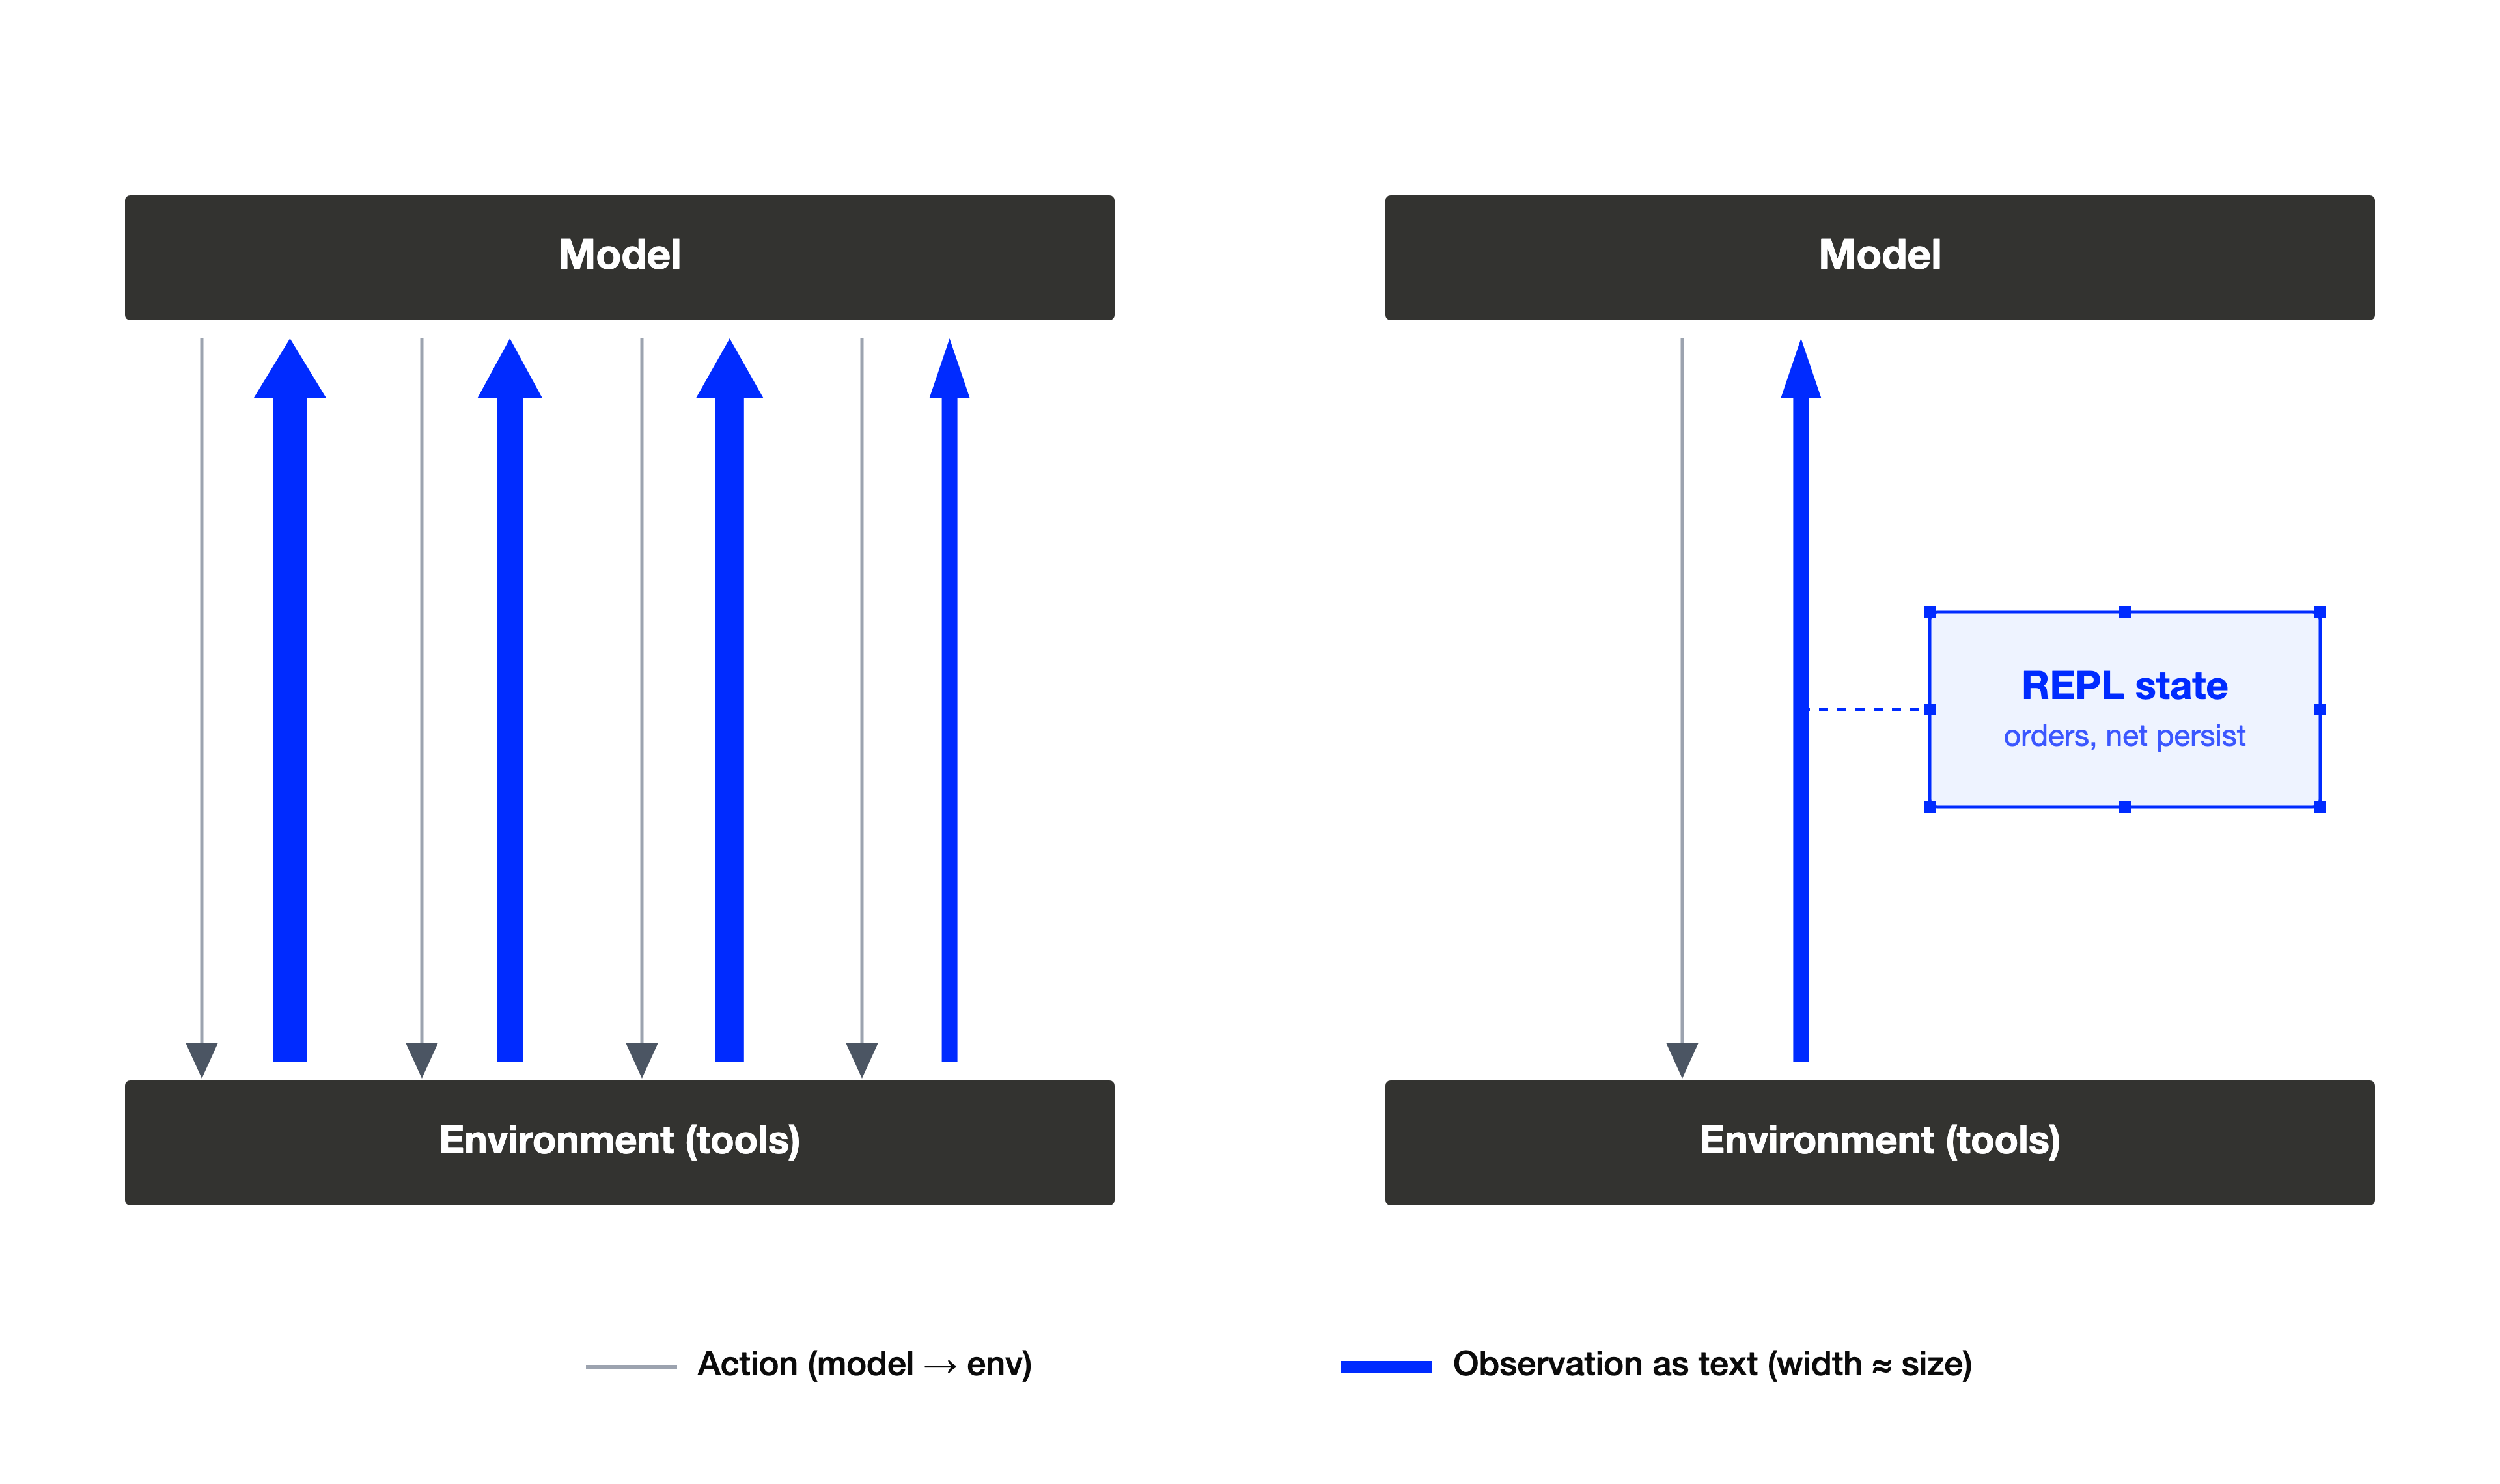
\includegraphics[width=0.9\textwidth]{figures/repl_executable_composition.png}
  \caption{\textbf{Executable composition.} Under function calling (left), each intermediate observation returns through the model as text: one round-trip per dependency step. In the REPL (right), dependent values persist in executable state (\texttt{orders}, \texttt{net}), so the same chain resolves in a single round-trip. Arrow thickness is observation size.}
  \label{fig:repl_composition}
\end{figure}

The second mechanism is \textbf{validated reuse}, which extends composition across tasks. Two operations govern a helper's lifecycle: \verb|save_tool| stages a self-derived helper into a candidate pool, and \verb|promote_tool| makes it callable by later queries, but only after it passes a private validation run against a held-out reference. Promotion after validation is the load-bearing ordering: a promoted helper is shared across a user's later sessions and is live in \mindforge{} rollouts (Section~\ref{sec:rsi_mindforge}), so promoting one unvalidated would turn a one-off local error into a standing fault across both serving and training. A promotion that later proves bad is logged and demoted, not silently retained.

Because promotion is scoped, a user's recurring workflow compiles into a validated helper in their own namespace, captured without a gradient step.

External services enter the namespace through a ToolProxy: Python-shaped wrappers carrying \verb|NoAI| visibility boundaries and retry semantics, so that a model-facing signature matches runtime behavior by construction, the tool-exposure contract of Section~\ref{sec:harness_hcp}~\citep{macaron_v1_blog2026}. \mindforge{} imports this same harness object rather than a stand-in, which forecloses train--serve tool drift at the source. The REPL is not universally best: stateful observe-before-commit APIs~\citep{patil2025berkeley} penalize committing several dependent calls blind, and independent shell tasks~\citep{terminalbench2026} give it nothing to compose; there the harness lets the L1 agent fall back to shell or discrete calls.

\subsubsection{Harness Context Protocol}
\label{sec:harness_hcp}

Real-world agent runs depend on configuration that is otherwise scattered across command-line flags, environment setup, local files, and runtime-specific defaults. The \hcp{} (HCP) is a versioned TOML contract for recreating that runtime from a portable, auditable artifact~\citep{hcp_sdk2026}. Its purpose is narrower and more operational than a generic ``context configuration'': an HCP producer writes a run specification, and a consumer resolves it in a deterministic order before creating the agent session.

The concrete surface HCP standardizes:
\begin{itemize}[leftmargin=*]
  \item \textbf{Runtime and model selection.} Working directory, backend, provider, model identifier, context window, generation limits, and provider options.
  \item \textbf{Action surface.} Tool allowlists, MCP servers, extensions, hooks, and the policies that control what the agent may invoke.
  \item \textbf{Context resources.} System prompts, \texttt{AGENTS.md}-style files, skills, prompt templates, embedded resources, and their deterministic materialization.
  \item \textbf{Session and workspace state.} Session snapshots plus optional workspace inputs, visibility, snapshot policy, and declared outputs.
  \item \textbf{Environment contract.} Required and optional environment names, path-resolution rules, and secret references without embedding portable credentials.
\end{itemize}

The current Python SDK operates in wrapper mode: it validates the outer configuration, asks \texttt{pi-hcp} to prepare the runtime, launches the ACP process, and manages a session through the Agent Client Protocol~\citep{hcp_sdk2026}. Full semantic validation and native Python materialization remain outside the SDK. In the RSI loop, HCP therefore serves as the versioned boundary between configuration search and execution.

It is worth being precise about what is and is not trainable here, because the two are easy to conflate. The protocol carries no gradients: an HCP artifact is a declarative TOML document, and no optimizer ever writes to it. What the model \emph{can} do is rewrite the harness the protocol describes. Because prompts, skills, tool allowlists, hooks, and workspace resources are all addressable fields in a portable artifact, a model version can propose edits to them, have the edits evaluated on a re-run of the affected slice, and ship the survivors as the next configuration, self-iteration of the harness conducted in language space rather than in parameter space (Section~\ref{sec:rsi_loop}). Neither half is sufficient alone. Configuration search moves in discrete jumps and cannot acquire a skill the base does not already have, though Section~\ref{sec:rsi_coverage} measures how much of what scores as a missing skill is an unelicited one; adapter training acquires skills but cannot reach the tool surface or the instructions that decide when to use them. Coupled through \mint{}, which parameterizes the specialists as LoRA revisions over a frozen base (Section~\ref{sec:infra_mint})~\citep{lu2026announcing}, the pair becomes one trainable system: a candidate HCP is what a rollout executes against, the resulting trajectories are what the adapters are trained on, and \mindforge{} ships the two as a linked model--configuration version. The trainable object is the model--harness pair, not the protocol.

\subsubsection{Live Harness Updates Enable Continual Learning}
\label{sec:harness_live}

Section~\ref{sec:mol_continual} described the frozen base and adapter registry as
an architectural affordance for continual learning. The harness supplies the
operational revision path: a new capability may first appear as a registered
tool, HCP configuration, \uifora{} component, or REPL helper promoted after
validation. When trajectory evidence warrants a parameter update, the change can
then be transferred into a specialist adapter. The present evaluation measures
the configuration-search stage, not repeated transfer across adapter generations.

This gives \macaron{} three release clocks: the base (tied to platform-level models such as GLM-5.2~\citep{glm52_2026,glm5_2026}), the specialists (updated through the RSI process in Section~\ref{sec:rsi}), and the harness. Harness changes do not require a weight update, so they can be evaluated and released on a shorter cycle than a new base or specialist revision.

\subsection{Recursive Self-Improvement}
\label{sec:rsi}

\macaron{} is improved through a versioned data-generation and training cycle rather than a fixed post-training corpus. The cycle runs against the production harness described above: a model version proposes tasks beyond its current competence, attempts them in an executable agent environment, and produces evaluated trajectories. Those trajectories support two different forms of improvement: language-space search over the runtime configuration, and parameter updates to the specialist adapters. \mindforge{} maintains the lineage connecting problem banks, evaluation runs, selected trajectories, training jobs, configurations, and model versions. This subsection describes the optimization object, the role of the framework, and the recursive self-improvement (RSI) cycle that connects them (Figure~\ref{fig:system_overview}).

\begin{figure}[t]
  \centering
  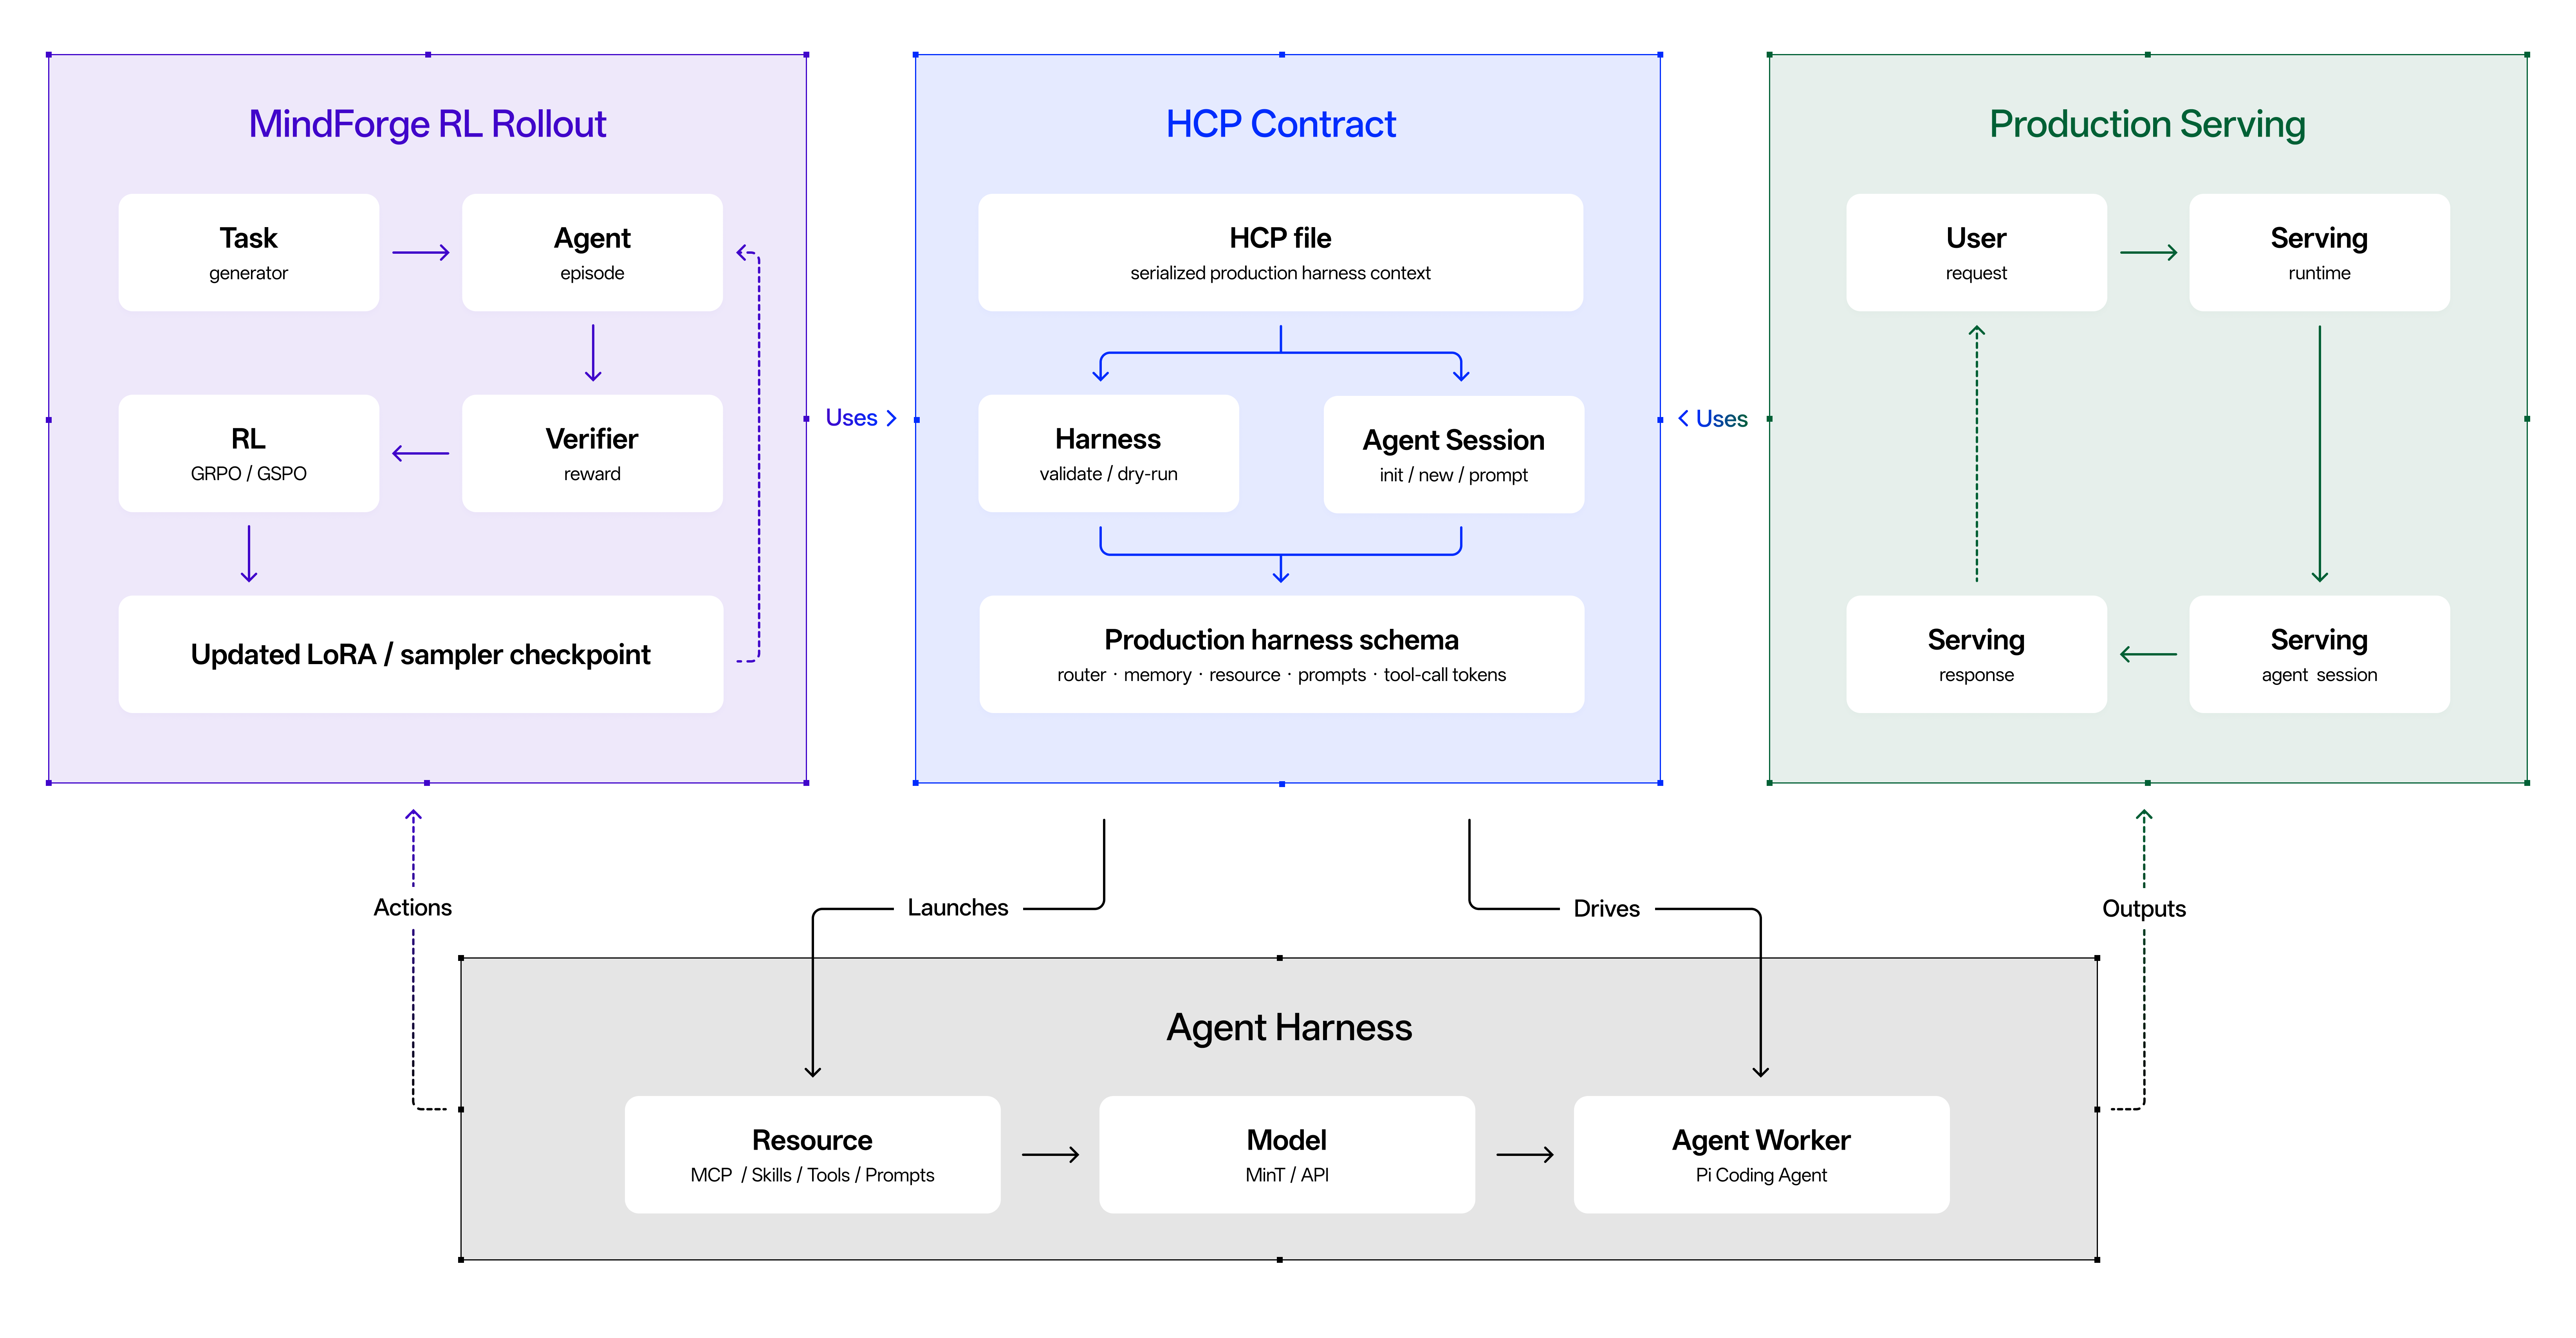
\includegraphics[width=\textwidth,height=0.4\textheight,keepaspectratio]{figures/system_overview.png}
  \caption{The three loops that share one harness. \mindforge{} runs RL rollouts against the same agent harness used for production serving; an HCP contract serializes the harness context (router, memory, resources, prompts, and tool-call tokens) so training and serving configurations can be compared explicitly. Matching the recorded contract makes configuration drift auditable but does not guarantee behaviorally identical executions.}
  \label{fig:system_overview}
\end{figure}

\subsubsection{Agent RL on a Frozen Sparse Base}
\label{sec:rsi_formulation}

Let \(\theta\) denote the parameters of the frozen sparse base, \(\phi\) the trainable LoRA parameters, and \(c\) a versioned harness configuration. The agent policy can be written as
\begin{equation}
  \pi_{\phi}(a_t \mid o_{\leq t}; \theta, c),
\end{equation}
where \(o_{\leq t}\) contains the conversation and observations exposed by the harness, and \(a_t\) is a model-visible action. An action may be a message, a clarification, a discrete tool call, or an expression evaluated by the stateful read--eval--print loop defined in Section~\ref{sec:harness_repl}. Adapter selection is a separate Proxy-mediated route hop (Section~\ref{sec:mol_router}), not a tool call made from this action space. The resulting episode is recorded as
\begin{equation}
  \tau=(o_0,a_0,\ldots,o_T,a_T,y),
\end{equation}
where \(y\) contains the task-level outcome and any process-level judgments attached by the evaluator.

This factorization distinguishes two update paths that are easy to conflate. Model optimization changes \(\phi\) while keeping \(\theta\) fixed; configuration search selects a new \(c\) without treating HCP as a learned parameter. The training backend uses GRPO~\citep{shao2024deepseekmath} to update the adapters from selected trajectories. Sparse-base rollout consistency and long-context execution are handled by the infrastructure in Section~\ref{sec:infrastructure}. This release reports the adapter training configuration (learning rate, batch size, epochs, schedule, and optimizer) in Appendix~\ref{app:training_details}.

The action substrate is part of \(c\), not an incidental wrapper. In the REPL substrate, dependent primitive operations execute inside a persistent namespace, so intermediate values need not be serialized through the model after every call~\citep{wu2026replharnesses}. For stateful APIs that require observing one result before committing the next action, the same runtime can instead expose discrete calls. The policy is therefore trained and evaluated against an explicit action interface rather than an abstract tool-use label.

\subsubsection{\mindforge: Lifecycle Orchestration}
\label{sec:rsi_mindforge}

\mindforge{} is the control plane of the RSI cycle. It manages problem banks, evaluation runs, conversion of evaluated trajectories into trainable datasets, training jobs, and a version registry that links each model to its parent, data, configuration, and evaluation results. Compute-heavy operations are delegated through pluggable benchmark and training backends. The control plane consequently defines lifecycle and provenance, while a backend defines the semantics of task execution, scoring, and optimization.

An HCP artifact provides the backend with a versioned runtime contract (Section~\ref{sec:harness_hcp})~\citep{hcp_sdk2026}. It records model and provider selection, tool policy, skills, prompts, MCP servers, hooks, session state, and workspace staging. The selected action substrate determines how model outputs become executable actions. Recording both artifacts makes a run reconstructable at the configuration boundary: train--serve differences can be inspected as differences in configuration, resources, or backend realization. This is a reproducibility contract, not a claim that two executions are behaviorally identical.

After each update, \mint{} exports the changed LoRA state as a serving-compatible adapter revision instead of moving or merging the frozen base; trajectories, rewards, and routing metadata remain separate rollout records (Section~\ref{sec:infra_mint})~\citep{lu2026announcing}.

This separation also keeps framework claims aligned with implementation. \mindforge{} does not redefine GRPO, the REPL, or HCP. It connects their artifacts into a stable lineage:
\[
  (\text{problem bank},\, \text{model},\, \text{HCP})
  \longrightarrow \text{evaluated trajectories}
  \longrightarrow (\text{dataset},\, \text{next model},\, \text{next HCP}).
\]
The lineage is the unit of an RSI generation. A model checkpoint without its problem-bank version, selected data, and runtime configuration is an incomplete record of the experiment.

\subsubsection{Three-Stage RSI Cycle}
\label{sec:rsi_loop}

\paragraph{Discovery.}
Starting from a versioned seed bank, the current model proposes harder task variants by lifting constraints, introducing hidden preferences, chaining sub-goals, or embedding contradictions. Each proposal must include either a verifiable answer or an evaluation rubric. Candidate tasks are retained only when they satisfy two complementary criteria: \emph{quality}, meaning that the task and its evaluation are well-defined, and \emph{learning value}, meaning that the current model does not already solve the task reliably. The verifier, difficulty estimator, and acceptance thresholds belong to the benchmark backend; \mindforge{} records the resulting bank and its provenance.

\paragraph{Expansion.}
The accepted tasks are executed by the current model under a fixed model--HCP pair. The evaluator scores both task outcome and relevant process behavior, producing a set of trajectories rather than a single answer corpus. Audits then localize failure to the model, the task, or the harness configuration. For example, an audit may reveal unnecessary model round-trips, an action that should have remained discrete, a missing tool boundary, or an instruction that causes premature routing. Candidate changes to prompts, skills, tool exposure, hooks, and other HCP-carried resources are evaluated by re-running the affected slice. Section~\ref{sec:rsi_coverage} reports what this search recovers on a set the base fails outright. Configuration changes are accepted on observed behavior rather than on prompt-author intuition; the acceptance gate is an automatic eval pass against the affected benchmark slice, with human review reserved for changes that touch tool exposure or safety-relevant boundaries.

\paragraph{Update.}
Trajectory selection filters invalid runs, removes duplicates, and retains examples that are both validated and informative for the next model. The selected trajectories become input to the training backend, which updates the LoRA specialists while the sparse base remains frozen. In parallel, the accepted HCP is registered as the runtime configuration of the next generation. \mindforge{} links the new adapter state and HCP to their parent artifacts and evaluation evidence. The resulting model--configuration pair returns to discovery, where its changed competence induces a new task distribution.

The three stages therefore form a feedback system. Discovery adapts the curriculum to the current policy; expansion searches behavior in the executable environment; update transfers validated behavior into parameters while preserving the configuration that produced it. Progress is measured across linked generations, not inferred from the existence of a later checkpoint.

\subsubsection{AutoResearch, Trajectory Selection, and Context Learning}
\label{sec:rsi_autoresearch}

The Preview report~\citep{macaron_v1_preview2026} described self-evolution through AutoResearch, trajectory selection, and what it called \emph{context learning} (validated-trajectory transfer, not in-context learning). In V1 these mechanisms are integrated into the three-stage cycle above.

\emph{AutoResearch} is language-space search inside expansion. The model proposes changes to prompts, skills, scaffolds, or tool-use policy; when represented by HCP resources, each proposal becomes a portable candidate configuration that can be executed and compared. AutoResearch changes the conditions under which behavior is elicited before changing the model weights; Section~\ref{sec:rsi_coverage} measures the reach of that change.

\emph{Trajectory selection} closes expansion by deciding which observed behaviors should influence the next model. A useful trajectory is not merely successful: it must be valid under the evaluator, attributable to the intended task and configuration, and sufficiently informative to justify inclusion. This selection step prevents configuration search, evaluator failures, and duplicated solutions from being indiscriminately distilled into the model.

\emph{Context learning} is the transfer from validated language-space behavior to the parameter update. Selected trajectories provide the training signal for the next adapters, while the accepted HCP remains a separately versioned artifact. Keeping these outputs distinct makes it possible to ask whether a gain came from weights, configuration, or their interaction. This release does not report that quantitative attribution; the controlled generation-by-generation comparison that would isolate it remains required.

\subsubsection{Expansion Coverage on a Base-Failure Set}
\label{sec:rsi_coverage}

The expansion stage searches configuration space against a fixed task set. We measure its reach on 122 simulation tasks grouped under 29 TerminalBench~2.1~\citep{terminalbench2026} source families, selected precisely because the frozen GLM-5.2-FP8 base scores every one of them not-pass under the official reward. The retained artifact does not include the per-family task counts. The base stays frozen throughout: no optimizer step is taken anywhere in the run, and every change is an edit to HCP-carried resources, task skills, tool exposure, or hooks. Because passing zero tasks was the selection criterion, the pre-sweep coverage is $0/122$ by definition, a selected failure slice rather than the base's TerminalBench pass rate.

Figure~\ref{fig:rsi_coverage} plots 69 chronological jobs, 450 task attempts in total ($3.69$ per task). Cumulative unique coverage reaches $122/122$ at job 69: each task passes at least once under one of the tested configurations without a weight update. Because a passing configuration was found for every task, failure under the baseline configuration does not by itself mean the behavior is absent from the frozen model. And because the search was adaptive, each job targeted the tasks still uncovered, so $122/122$ is a coverage ceiling under adaptive configuration selection, not a held-out estimate of how any single configuration generalizes.

One configuration does not get there. Jobs 11 and 12 sweep the full set under a single portfolio configuration each and pass $4/122$ ($3.3\%$) and $11/122$ ($9.0\%$); 97 of the run's 109 harness errors fall in those two jobs. What follows is not more sampling from that distribution. Targeting the families still uncovered yields a pooled pass rate of $64.5\%$ over 36 skill-and-HCP jobs, and the final 21 jobs with stop-gate hooks yield $81.2\%$ while closing the remaining 62 tasks with 3 errors (Table~\ref{tab:rsi_coverage}). The ratio between the final phase and the two full-set sweeps is $13\times$ in per-attempt yield. Because the task mix, targeting policy, and harness-error rate differ between phases, this ratio describes the search trajectory rather than isolating a causal effect of the added hooks.

The two numbers illustrate the intended division of labor between the update paths of Section~\ref{sec:rsi_formulation}. The better of the two full-set configurations reaches $9\%$ of this set; adaptive search over $c$ eventually covers all of it at $3.69$ attempts per task. The role assigned to the subsequent $\phi$ update is to transfer selected behavior into an adapter, but this experiment does not execute that update or measure whether the transfer generalizes.

% figures/rsi/rsi_coverage.tex -- GENERATED, do not hand-edit.
% Source: experiments/glm52-zero-source-skill-portfolio/runs/reports/
%         passrate_history/not_pass_sim_passrate_history.json
% Generator: tools/gen_rsi_fig.py
% Denominator: 122 simulation tasks (29 zero-coverage TB2.1 source families).
% Model frozen throughout (GLM-5.2-FP8); only the Claude-HCP harness varies.
\begin{figure}[t]
\centering
\begin{tikzpicture}

%% ---------- panel A: cumulative unique coverage ----------
\begin{axis}[
    name=cov,
    height=4.6cm,
    width=0.93\textwidth,
    axis line style={mindlabmuted},
    tick style={mindlabmuted},
    label style={font=\small, color=mindlabink},
    tick label style={font=\footnotesize},
    grid=major, grid style={mindlabgrid, dashed},
    axis on top,
    xmin=0, xmax=70,
    ymin=0, ymax=104,
    clip=false,
    ylabel={Cumulative coverage (\%)},
    xticklabels={},
    ytick={0,20,40,60,80,100},
]
\fill[mindlabmuted!14] (axis cs:0.5,0) rectangle (axis cs:10.5,104);
\fill[mindlabmuted!8] (axis cs:10.5,0) rectangle (axis cs:12.5,104);
\fill[mindlabbluepale!55] (axis cs:12.5,0) rectangle (axis cs:48.5,104);
\fill[mindlabbluepale] (axis cs:48.5,0) rectangle (axis cs:69.5,104);
\node[anchor=north, font=\scriptsize, color=mindlabink, inner sep=1pt] at (axis description cs:0.5,-0.035) {\textbf{Jobs:} 1--10 Retry control \quad 11--12 Portfolio v1 sweep \quad 13--48 Skill/HCP search \quad 49--69 + Stop-gate hooks};
\addplot[mindlabblue, mark=*, mark size=1.25pt, line width=0.9pt]
  coordinates {
    (1,0.0)(2,0.0)(3,0.82)(4,0.82)(5,0.82)(6,0.82)
    (7,1.639)(8,1.639)(9,1.639)(10,1.639)(11,4.918)(12,11.475)
    (13,11.475)(14,11.475)(15,13.115)(16,13.115)(17,13.115)(18,13.115)
    (19,13.115)(20,13.934)(21,14.754)(22,15.574)(23,18.033)(24,20.492)
    (25,21.311)(26,22.131)(27,22.131)(28,22.951)(29,23.77)(30,24.59)
    (31,25.41)(32,26.23)(33,27.049)(34,27.049)(35,27.869)(36,28.689)
    (37,29.508)(38,30.328)(39,31.148)(40,31.967)(41,36.885)(42,40.984)
    (43,40.984)(44,42.623)(45,46.721)(46,47.541)(47,49.18)(48,49.18)
    (49,53.279)(50,59.016)(51,59.836)(52,63.934)(53,64.754)(54,66.393)
    (55,68.033)(56,69.672)(57,71.311)(58,72.951)(59,74.59)(60,75.41)
    (61,76.23)(62,77.869)(63,82.787)(64,83.607)(65,84.426)(66,89.344)
    (67,96.721)(68,99.18)(69,100.0)
  };
\end{axis}

%% ---------- panel B: per-job pass rate on attempted tasks ----------
\begin{axis}[
    name=rate,
    at={(cov.south west)}, anchor=north west, yshift=-0.75cm,
    height=3.9cm,
    width=0.93\textwidth,
    axis line style={mindlabmuted},
    tick style={mindlabmuted},
    label style={font=\small, color=mindlabink},
    tick label style={font=\footnotesize},
    grid=major, grid style={mindlabgrid, dashed},
    axis on top,
    xmin=0, xmax=70,
    ymin=0, ymax=108,
    xlabel={Chronological job step},
    ylabel={Pass rate on\\attempted tasks (\%)},
    ylabel style={align=center},
    ytick={0,25,50,75,100},
]
\fill[mindlabmuted!14] (axis cs:0.5,0) rectangle (axis cs:10.5,108);
\fill[mindlabmuted!8] (axis cs:10.5,0) rectangle (axis cs:12.5,108);
\fill[mindlabbluepale!55] (axis cs:12.5,0) rectangle (axis cs:48.5,108);
\fill[mindlabbluepale] (axis cs:48.5,0) rectangle (axis cs:69.5,108);
\addplot[only marks, mark=*, mark size=1.15pt, color=mindlabmuted, opacity=0.75]
  coordinates {
    (1,0.0)(2,0.0)(3,20.0)(4,20.0)(5,20.0)(6,0.0)
    (7,20.0)(8,20.0)(9,20.0)(10,0.0)(11,3.28)(12,9.02)
    (13,0.0)(14,0.0)(15,66.67)(16,0.0)(17,0.0)(18,0.0)
    (19,0.0)(20,100.0)(21,50.0)(22,100.0)(23,100.0)(24,100.0)
    (25,100.0)(26,33.33)(27,100.0)(28,100.0)(29,100.0)(30,100.0)
    (31,100.0)(32,100.0)(33,100.0)(34,0.0)(35,100.0)(36,100.0)
    (37,100.0)(38,100.0)(39,100.0)(40,100.0)(41,100.0)(42,100.0)
    (43,66.67)(44,100.0)(45,83.33)(46,100.0)(47,28.57)(48,0.0)
    (49,100.0)(50,100.0)(51,14.29)(52,83.33)(53,100.0)(54,100.0)
    (55,100.0)(56,100.0)(57,100.0)(58,100.0)(59,100.0)(60,50.0)
    (61,100.0)(62,100.0)(63,85.71)(64,100.0)(65,100.0)(66,85.71)
    (67,69.23)(68,85.71)(69,100.0)
  };
\draw[mindlabblue, line width=1.4pt] (axis cs:0.5,12.00) -- (axis cs:10.5,12.00);
\draw[mindlabblue, line width=1.4pt] (axis cs:10.5,6.15) -- (axis cs:12.5,6.15);
\draw[mindlabblue, line width=1.4pt] (axis cs:12.5,64.47) -- (axis cs:48.5,64.47);
\draw[mindlabblue, line width=1.4pt] (axis cs:48.5,81.25) -- (axis cs:69.5,81.25);
\node[anchor=south, font=\scriptsize\bfseries, color=mindlabblue, inner sep=1.5pt] at (axis cs:5.5,12.00) {12.0\%};
\node[anchor=south, font=\scriptsize\bfseries, color=mindlabblue, inner sep=1.5pt] at (axis cs:11.5,6.15) {6.1\%};
\node[anchor=south, font=\scriptsize\bfseries, color=mindlabblue, inner sep=1.5pt] at (axis cs:30.5,64.47) {64.5\%};
\node[anchor=south, font=\scriptsize\bfseries, color=mindlabblue, inner sep=1.5pt] at (axis cs:59.0,81.25) {81.2\%};
\end{axis}

\end{tikzpicture}
\caption{\textbf{Expansion over a base-failure set.} 122 simulation tasks from 29
TerminalBench~2.1 source families the frozen GLM-5.2 base fails under the official
reward. \textbf{Top:} cumulative unique coverage, reaching $122/122$ at job 69.
\textbf{Bottom:} each job's pass rate on the tasks it attempted, with the pooled
rate per phase in blue. The model is frozen throughout; only the HCP-carried harness
changes. Jobs 11--12 sweep the full set under one configuration each; later jobs target
the families still uncovered.}
\label{fig:rsi_coverage}
\end{figure}

\begin{table}[t]
\centering
\caption{Phase breakdown of the 69-job expansion run of Figure~\ref{fig:rsi_coverage}. Attempts count task trials, so a job sweeping the full set contributes 122. Pooled rate is passes over attempts within the phase; coverage is the cumulative unique tasks passed at the end of it, against the fixed denominator of 122. The model is frozen throughout.}
\label{tab:rsi_coverage}
\footnotesize
\setlength{\tabcolsep}{5pt}
\begin{tabular}{llrrrrr}
\toprule
Phase & Jobs & Attempts & Passes & Pooled & Errors & Coverage \\
\midrule
Retry control        & 1--10  & 50  & 6  & $12.0\%$ & 6  & $2/122$ \\
Portfolio v1 sweep   & 11--12 & 244 & 15 & $6.1\%$  & 97 & $14/122$ \\
Skill/HCP search     & 13--48 & 76  & 49 & $64.5\%$ & 3  & $60/122$ \\
$+$ Stop-gate hooks  & 49--69 & 80  & 65 & $81.2\%$ & 3  & $122/122$ \\
\midrule
Total                & 1--69  & 450 & 135 & $30.0\%$ & 109 & $122/122$ \\
\bottomrule
\end{tabular}
\end{table}

\FloatBarrier
